\song{Pramínek vlasů (Suchý, Šlitr)}
%Mara_2017_01_19

\setlength{\columnsep}{-2cm}
\begin{multicols}{2}
\ve{}
Když měsíc \ch{D}rozlije \ch{Hmi}světlo své \ch{Emi}po kra\ch{A7}ji\\
a hvězdy \ch{D}{ř}eknou, \ch{Hmi}{ž}e čas je jít \ch{Emi}spát, \ch{A7}\\
pramínek \ch{D}vlasů \ch{Hmi}jí ustřihnu \ch{Emi}potají, \ch{A7}\\
komu -- no \ch{D}přece té, \ch{G7}kterou mám \ch{D}rád. \ch{A7}

\ve{}
Pramínek vlasů jí ustřihnu potají,\\
já blázen pod polštář chci si ho dát,\\
ačkoliv sny se mi zásadně nezdají,\\
věřím, že dnes v noci budou se zdát.

\cho{}
O sny mě \ch{C}připraví teprve \ch{D}svítání,\\
zpěv ptáků v \ch{C}oblacích a modré \ch{D}nebe,\\
od vlasů, \ch{G7}jichž jsem se dotýkal \ch{D}ve spaní,\\
nový den \ch{B\guitarFlat{}7}nůžkama odstřihne \ch{A7}tebe.

\ve{}
Na bílém polštáři, do kroužku stočený,\\
zbude tu po tobě pramínek vlasů,\\
nebudu vstávat, dál chci ležet zasněný,\\
je totiž neděle a mám dost času,\\
\ch{Hmi}je totiž \ch{Emi}neděle \ch{A7}a mám dost \ch{D}{č}asu.

\cho{}
~

\vfill
\columnbreak


\begin{flushright}
\vspace*{\fill}
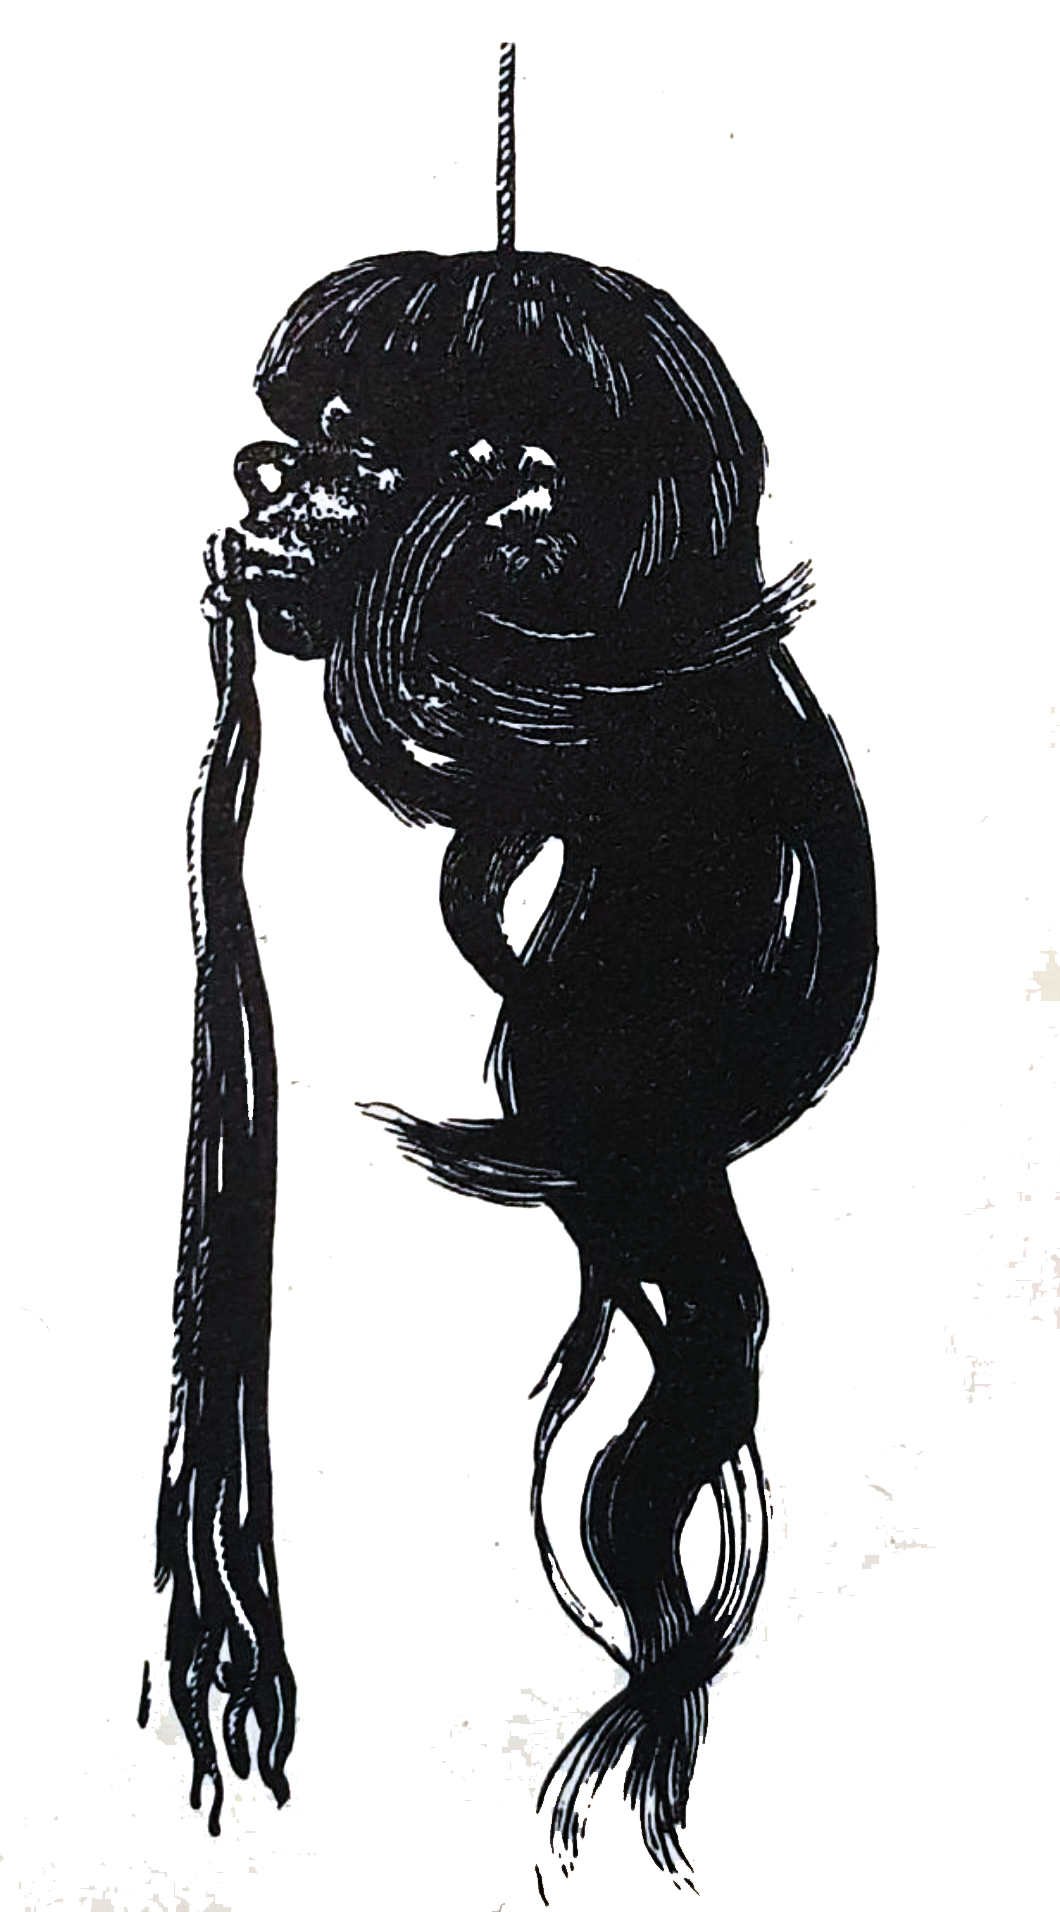
\includegraphics[width = 0.8\columnwidth]{images/_praminek_vlasu.png}
\vspace*{\fill}
\end{flushright}

\end{multicols}
\esong
\setlength{\columnsep}{0.5cm}